\documentclass[12pt]{article}
\usepackage{graphicx}% Include figure files
\usepackage[utf8]{inputenc}
\usepackage{float}
\usepackage{chngcntr}
\counterwithin{table}{section}
\counterwithin{figure}{section}
\usepackage[left=1.25in, right=1.25in, top=1in, bottom=1in]{geometry}
\usepackage{float}

\usepackage{parskip}


\begin{document}

%
% Title Page
%
\begin{titlepage}
\title{ Learning About and Building a Computer Cluster Using Recently Retired Server-Grade Computers \vspace{+2ex}}

\author{\large Matthew Muller, Maxwell Herron, Nathaniel Seleshi,
Mohamad Omar,\\ Hana Keinan, Scott Kerlin, Erik Steinmetz}

\date{\parbox{\linewidth}{\centering%
  \large
  Computer Science Department\\
  Augsburg University\\
  2211 Riverside Ave, Minnepaolis, MN, 55454\\
  mullermm@augsburg.edu, herronm@augsburg.edu, seleshin@augsburg.edu, omarmm@augsburg.edu, keinanh@augsburg.edu, kerlin@augsburg.edu, steinmee@augsburg.edu}}
  
\maketitle
\thispagestyle{empty}

%
% Abstract
%
\section*{\Large \hfil Abstract \hfil}

In 2019, there exists an excess of server-grade computers capable of performing large computational tasks. Currently, you can purchase a 7-year-old server for under \$200. The equilibrium point of computational capability and price of this older hardware makes it possible to learn how to create a computer cluster with a small initial investment. A computer cluster is a group of computers linked together to act as one logical unit, or single computer. This led us to as the following question: Using recently retired, high performance hardware, can we learn to build a cluster that is computationally comparable to current hardware for a relatively reduced price?

\end{titlepage}

%
%Overview
%
\section{\Large Overview}

\subsection{Parallel computing and its importance}

Parallel computing originally came about in the 1950's alongside the development of supercomputers. With the advancement of computer hardware lifting limitations, parallel computing has only gained in popularity. In the late 1980's, parallel computing became commonplace with the invention of computer clusters. 

Parallel computing is the foundation of what makes a cluster effective. By breaking down large tasks into sub-jobs, and then handing those jobs to various processors, large jobs can quickly be completed. This type of computing is what makes clusters effective.


\subsection{Time line of the building process}
\begin{table} [htb!]
    \centering
    \begin{tabular}{ll}
        Week 1 & Purchase necessary materials   \\
        Week 2 & Physical assembly of cluster   \\
        Week 3 & Connect and configure network  \\
        Week 4 & Install and configure operating system \\
        Week 5 & Setup MPI and benchmark    \\
        Week 6 & Analyze data and compose paper    \\
    \end{tabular}
    \caption{Building process time line}
    \label{tab:timeline}
    
\end{table}

The process of constructing and analyzing the cluster took about six weeks. Table \ref{tab:timeline} is an overview of what tasks were completed each week. While the project only took 6 weeks to complete, it could be expanded to take more time to finish. This might be beneficial if a project like this was expanded into a course. Section \ref{sec:expansion} speaks more about how this project could be expanded.

\subsection{Technical specs and architecture}

The specs of the cluster are displayed in Table \ref{tab:clusterspecs}, which is made up of 6 computers. All of the nodes in the cluster are completely homogeneous with one exception: the head node. The head node has 960GB of storage space while the child nodes have 240GB of storage. The head node has increased storage because it holds the folder where the files to be processed is stored. This folder is then mounted to the child nodes using the network file system protocol.

% Specs of whole cluster
\begin{table} [H]
    \centering
    \begin{tabular}{l|c|c|c|c|c}
        Node & Quantity & Ind. RAM & Total RAM & Ind. Storage & Total Storage\\
        \hline
        Head & 1 & 48GB & 48GB & 960GB & 960GB \\
        Child & 5 & 48GB & 240GB & 240GB & 1200GB\\
        \hline
        Cluster & 6 & - & 288GB & - & 2160GB\\
    \end{tabular}
    \caption{Technical specs of entire cluster}
    \label{tab:clusterspecs}
\end{table}

Each computer in the node is a dual processor machine, with each processor having its own RAM. Figure \ref{fig:cpuarc} is a visual representation of the architecture of one node. Table \ref{tab:nodespecs} is the list of technical specs for one specific node in the cluster. Again, the head node has 960GB of storage instead of 240GB. 

% Specs of one node
\begin{table} [H]
    \centering
    \begin{tabular}{l c l|l}
        Component & Quantity & Specific Part & Total\\
        \hline
        Mother Board & 1 & HP Proliant DL360 G7 & -\\
        CPU & 2 & Intel Xeon X5670 & -\\
        RAM & 6 & HP 8GB 2Rx4 PC3-10600R & 48GB\\
        Storage & 2 & Kingston SSD & 240GB\\
    \end{tabular}
    \caption{Technical specs of entire cluster}
    \label{tab:nodespecs}
\end{table}

% Figure of the architecture of one node
\begin{figure} [H]
    \centering
    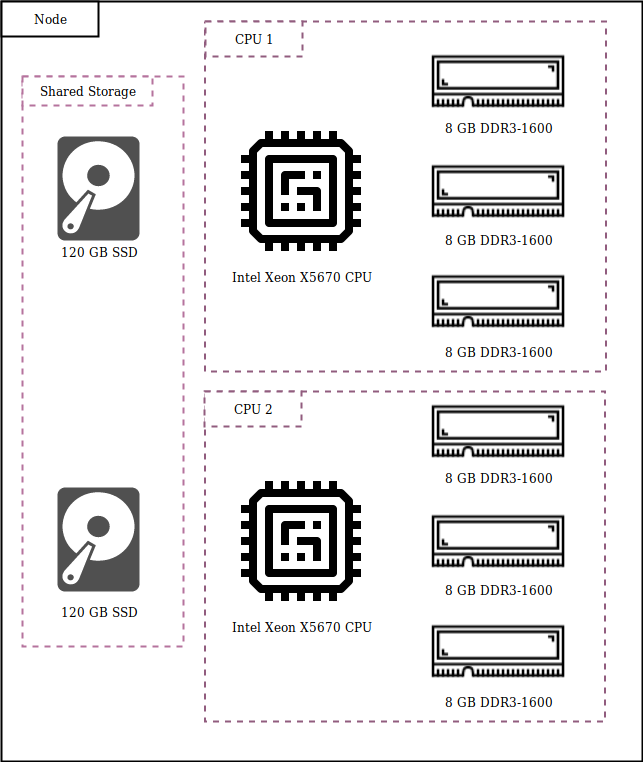
\includegraphics[width=0.7\textwidth, height=0.5\textheight]{CPUArch.png}
    \caption{Architecture of one Node}
    \label{fig:cpuarc}
\end{figure}

%
% Procurement of Parts
%
\section{Procurement of Parts}

\subsection{Donation of servers by Free Geek Twin Cities}
Free Geek Twin Cities is a non-profit electronic waste recycler who's mission is to help reduce electronic waste while rebuilding computers to sell to the community at a greatly reduced price. They were very kind and helped us make this cluster a reality.

Although this project can be completed for a reasonable price, Free Geek sold us the 6 HP Proliant G7 DL360 servers we used for \$250. This a discounted of about \$500. Free Geek also sold us a Netgear N900 Wireless N router and a 3COM Baseline Gigabit switch for \$5 a piece, saving us an additional \$20.

\subsection{Compatibility of parts}
For our servers, we needed to verify the parts we purchased would be compatible with the servers we had. Documentation \cite{HP} for the servers was easy to find and was a great resource to learn about compatibility. Using the HP documentation, we found what processors would be compatible and what RAM would be accepted by the mother board. This information is very important because not all RAM and processors are interchangeable on older hardware.

Learning about compatibility taught us a lot about different types of hardware and how the hardware works. We learned about different types of RAM (e.g., ECC, DDR) and RAM specs like voltage, bus speed, and data width. Also, we learned about technology that exists in the processors like hyper threading, Intel VT, and cache. Building this cluster forced us to dig deep into the hardware and figure out what parts and technology would be accepted or rejected by our servers.

\subsection{Required parts}

The servers we received from Free Geek Twin Cities were functional, but they did not contain RAM or storage mediums. Additionally, we decided to upgrade the CPUs to the Intel Xeon X5670 because the price point of about \$18.00 and good performance made it a quality upgrade for a low cost.

The servers we used were HP Proliant G7 DL360 servers, which required hard drive caddies to hold the storage mediums. Each server had 6 to 8 caddie slots and each slot needed a caddie in order for the fans to operate correctly and for the airflow to be correct. This meant we needed to purchase 34 caddies to fill the front of each server.

Constructing a cluster also requires some additional parts that can be overlooked if you don't take the construction process into account. For example, most the servers came with one processor and heat sink, but we were expanding them to have two upgraded processors each. We knew we would have to purchase two processors for each computer, but almost neglected the fact we needed to purchase an additional heat sink for the second processor socket. We caught this mistake by going through a dry run of the build process before we ordered parts. This helped us to see what we would need to purchase, identify any missed components, and get a feel for the build process.

\subsection{Pricing of parts we used}

All of the parts, except for the ones donated by Free Geek Twin Cities, were purchased from eBay.com \cite{eBay}. We found the eBay marketplace to have the lowest prices and also have the quantity of parts we needed.

Table \ref{tab:partlist} shows everything we needed to purchase to complete the cluster. Our total expenditures were \$1710.93. This is taking into account the donations by Free Geek Twin Cities. Table \ref{tab:freegeekdif} shows the eBay pricing in relation to the price we paid at Free Geek. Also, we did have some excess parts: 4 server fans, 14 sticks of 8GB ram, 3 tubes of thermal paste. We did this because buying a larger amount on eBay lowered the price point per item and gave us increased stock in case we wanted to expand the project later.

% Price list of parts purchased
\begin{table}[ht!]
    \centering
    \begin{tabular}{lcrr}
        Part Purchased &  Quantity &  Ind. Price & Item Total\\
        \hline
        HP Proliant G7 DL360 Servers & 6 & \$41.66 & \$250\\
        Additional HP Proliant Processor Fan & 10 & \$5.99 & \$55.99\\
        Intel X5670 Xeon Processors & 14 & \$18.20 & \$254.75\\
        1U Xeon Processor Heat Sinks & 5 & \$7.00 & \$35.00\\
        Tube Thermal Paste For Processors &	5 &	\$6.17 & \$30.85\\
        RAM - HP 8GB 2Rx4 PC3-10600R &	50 & \$11.00 & \$550.00\\
        HP Proliant G7 Hard Drive Caddy & 34 & \$7.00 &	\$146.99\\
        Kingston A400 120 GB SSD & 18 & \$19.99 & \$359.82\\
        3COM Baseline Switch 2920-SFPPlus & 1 & \$5.00 & \$5.00\\
        Netgear N900 Wireless N Router & 1 & \$5.00 & \$5.00\\
        Cat 6 Network Cable 2 Foot & 7 & \$1.75 & \$12.25\\
        90\% Isopropanol Alcohol & 1 & \$1.79 & \$1.79\\
        16GB USB Flash Drive & 1 & \$3.49 & \$3.49\\
        \hline
        Total & - & - & \$1710.93\\
    \end{tabular}
    \caption{Pricing of parts used}
    \label{tab:partlist}
\end{table}

% Difference of price between Free Geek and eBay
\begin{table}[ht!]
    \centering
    \begin{tabular}{lccc}
        Parts Purchased & Free Geek & eBay  & Difference\\
        \hline
        HP Proliant G7 DL360 Servers & \$250 & \$720 & \$470\\
        3COM Baseline Switch 2920-SFPPlus & \$5 & \$15 & \$10\\
        Netgear N900 Wireless N Router & \$5 & \$15 & \$10\\
        \hline
        Total & \$260 & \$750 & \$490\\
    \end{tabular}
    \caption{Price difference between Free Geek donations and eBay}
    \label{tab:freegeekdif}
\end{table}

What does this all mean? This means if we were to replicate this cluster using pure eBay pricing, we would have to pay \$2200.93. But, this cluster can be customized for many configurations. For example, you could reduce the price by \$286 by reducing the RAM to 16 GB per CPU instead of 24GB and not buying an extra 14 sticks. In all, you can expect to pay about \$2000 to replicate this cluster.

% Hardware Assembly
\section{Hardware Assembly}

One of the best parts of this project was getting the chance for each team member to learn how to assemble a computer. There were 5 team members and 6 computers, enabling each member to assemble a computer by themselves start to finish.

The actual hardware assembly process was simple. The process taught us how to install cooling fans, drop CPUs, apply a heat sink with thermal paste, install RAM, and install storage devices. Two members were well versed in computer hardware assembly, but the other three had never performed any of these task. The assembly process taught us about the architecture of a modern computer and was easy to perform.

Anytime we had a question about computer assembly, we referred to the documentation or to YouTube. The documentation was a great initial resource, but having YouTube \cite{YouTube} to visually see how to install a component into a computer was very beneficial. The ability to watch someone work with computer hardware was invaluable when it came to troubleshooting questions during the assembly process.

The hardest part of assembly was installing the processors. During the installation process, we realized one of the socket pins was bent and touching the adjacent pin. Using a razor blade, we successfully bent the pin back into place. This process was nerve racking considering any slip would render the server motherboard worthless. Getting the processors seated into the system was the most difficult part of assembling the servers.

%
% Networking
%
\section{Networking}

\subsection{Overview}

For ideas on how to network this cluster, we referenced a guide written by Serrano Pereira in 2013 \cite{pereira_2013}. This guide explained some ideas of how to network the computers physically, showed us how to install necessary software, and described how to edit files to get the machines to communicate together. The guide gave us good insight on how a cluster communicates inside a network.

\subsection{DHCP}

The way the computers in the cluster communicate with each other is by using the TCP/IP \cite{ibm}  protocol over a network. This means each computer has an IP address assigned to it so it can send and receive messages. The problem with connecting computers together with a switch is that the computers have no idea of what their IP address is or how to communicate to any adjacent computers. To solve this problem you use the Dynamic Host Configuration Protocol, or DHCP \cite{dhcp}.

User datagram protocol, or UDP, is another protocol used to move traffic across a network \cite{cisco}. While UDP has some advantages over TCP/IP, like the ability to define packet size, it also has some disavantages. First off, UDP does not guarantee a packet received packet will be sent. This is an important feature if you want to verify the information you sent was actually recived. Secondly, some software requires TCP/IP. It is for these two reasons we decided against using UDP. 

We found that most cluster projects set up the DHCP server, the process that assigns and manages computer IP addresses on a network, on the head node. We though about doing this, but decided that we would like to keep processing on the cluster exclusive to task related to the job being run and not networking management. Instead, we used a router to set up the DHCP server. Our router, and most routers today, have a web interface which make assigning static IP addresses to machines simple and easy.

One might ask why we need to have a router assign static IP addresses when we could just use a host table assigned to each computer. The reason we have the router handle this is so the cluster network appears as 1 IP address to anything outside of the cluster. This enables each server to be able to talk to any computer on the internet 

Another benefit of having the router separate form the head node is any communication between the cluster and the nodes will be managed by a device that is not actually part of the cluster. This theoretically decreases the computation time of a task on the head node. While we did not have time to test this configuration against putting the DHCP server on the head node, we believe that using dedicated hardware for a dedicated service is beneficial to overall performance.

\subsection{Network Topology}

\begin{figure} [!htb]
    \centering
    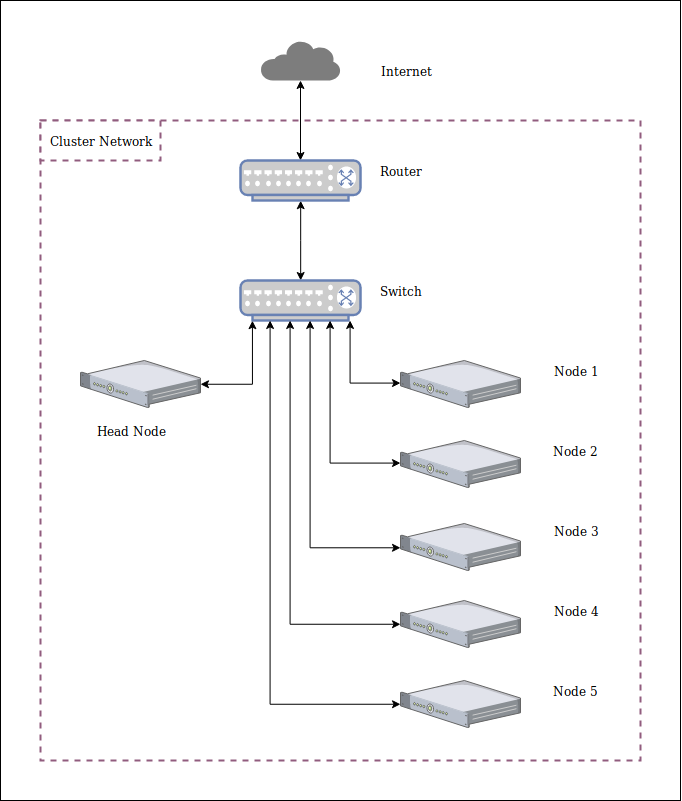
\includegraphics[width=0.8\textwidth, height=0.55\textheight]{NetworkDiagram.png}
    \caption{Network diagram of cluster}
    \label{fig:network}
\end{figure}

Our network is made up of 6 servers, the head and 5 nodes, connected to a switch. Our switch is a managed switch that remembers what the IP address of all the servers connected to it. The router that hosts the DHCP server is also connected to the switch, enabling the assignment of the IP addresses to all of the computers. Additionally, the router is connected to the internet. Figure \ref{fig:network} is a visual representation of the topology of this network.

One major benefit of having a router manage the DHCP instead of the head node is we can verify the cluster itself is assigned one IP address by the network we connected the cluster to. The reason this is beneficial is because all traffic between the servers is maintained inside of the cluster network and not passed to the larger network we connected to. As you can see in Figure \ref{fig:network}, all communications between the servers will stay on the cluster network, unless that communication requires to talk to the internet. Letting the traffic between the servers make it to the network outside of the cluster network is unnecessary, inefficient, insecure, and will most likely anger the network administrator of that network.

Having a good switch is also beneficial to an efficient system. Our switch has plenty of features that enable fast communication, but most importantly it is managed and communicates at gigabit speeds. A managed switch remembers the IP addresses of the computers attached to it, decreasing the number of hops it takes for one node to speak to another node. The switch will direct local traffic directly from one node to another without having to talk to the router. 

The time required to for a node to speak with another node is fast inside of our network. Table \ref{tab:ping} shows the average of 25 pings between the head node and each child node. The time for the head to speak with a node is measured in microseconds, a time we felt was very efficient.

\begin{table}[htb!]
    \centering
    \begin{tabular}{lrr}
        Node  &   Avg. Ping in Milliseconds  &  Avg. Ping in Microseconds\\
        \hline
        Head (Loopback) &   0.019ms     &   19$\mu$\\
        Node 1          &   0.161ms     &   161$\mu$\\
        Node 2          &   0.212ms     &   212$\mu$\\
        Node 3          &   0.217ms     &   217$\mu$\\
        Node 4          &   0.209ms     &   209$\mu$\\
        Node 5          &   0.163ms     &   163$\mu$\\
    \end{tabular}
    \caption{Average ping from head node}
    \label{tab:ping}
\end{table}

%
% Installing the operating system
%
\section{Installation of Software}

\subsection{Overview}

We again referenced the guide written by Serrano Pereira to install the specific software needed to get the cluster operational \cite{pereira_2013}. Specifically, the guide explained how to configure SSH, network file system, message passing interface, and the host files. This guide directly gave us the tools we needed to get the cluster software operational.

\subsection{Setting up the storage mediums and RAID}

The architecture for our nodes were homogeneous, except for the head node. The head had additional storage because we were going to virtually mount a folder from the head node to all of the children node. Mounting this folder means all the nodes will have access to the folder remotely. For this reason we decided to have the head node storage be formatted as a RAID.

A redundant array of independent disks, or RAID, is a way in which to organize data on storage mediums to prevent data loss \cite{raid}. Data is stored in arrays and these arrays have duplicate copies stored in multiple locations on storage mediums. This means that if a storage medium is lost, a duplicate of that information is saved elsewhere. In this scenario you can replace the bad storage medium and restore the RAID array without losing any data. The trade off for using a RAID is since data is duplicated, the total storage capabilities of the array are lowered.

We decided to have the head node be a RAID 5+0 because that is where the data being computed is stored. We wanted to be able to keep the cluster online and operational in case of a storage medium failure. It would be unfortunate to have the cluster process a 30 hour job only to have a storage medium fail in the last few hours and have to perform the entire computation again. Having a RAID 5+0 setup prevents this failure from stopping the cluster from finishing its job.

The child nodes were also set up in a RAID, but as a RAID 0. This means that the storage mediums act together as one logical drive, but there is no data duplication. We did this because we had multiple drives but only wanted one partition for the operating system.

The last thing to note is that server grade equipment typically has RAID controllers built into them. We were able to use the RAID controllers in our servers to create these logical drives via the BIOS menu. This is advantageous because if we let the operating system manage the RAID, we could potentially slow the CPU down. Having the RAID controller manage the reading and writing of data potentially increases the computational power of the cluster. 

\subsection{Installing the operating system}

The operating system we decided to use was Ubuntu Server 18.04 LTS. Ubuntu is a free flavor of Linux and is supported very well. The server version is geared towards running a computer as a server instead of a general purpose computer. This means things such as a graphical user interface are not installed while things such as openSSH server are. Additionally, there is a lot of support and documentation online for Ubuntu. It is for these reasons we decided on Ubuntu.

Installing Ubuntu was quite simple. We used a 16 GB USB flash drive to create an installation and ran it on all 6 computers. The only difference between each installation was naming each computer (e.g, Head, Node1, etc.) The process for installing Ubuntu is straight forward and streamlined by the installer.

\subsection{Installing message passing interface}

Message passing interface, or MPI, is a standard used to pass instructions between nodes in a parallel computing network \cite{mpidef}. This is the software used to actually execute jobs on the cluster. We chose to use hydra-3.3 \cite{mpi} to manage and execute jobs. This is different than open MPI \cite{openmpi}, an arguably more popular MPI. After experimentation, we found hydra to be more compatible with our system.

Configuring MPI is not complicated, but understanding how to execute jobs took time. For example, we had to make a host file containing all of the nodes we wanted MPI to execute on. We believe setting up MPI is system dependent and understanding how to use it can be a time consuming process.

%
%Bench marking
%
\section{Bench marking}

\subsection{Overview}

Bench marking is a way in which you can measure a computers performance capabilities in relation to another machine. A benchmark is a taxing job that is performed on a computer to see how fast that computer can complete the job. Once the job is complete, you can compare results with how well the taxing job was performed on a different machine. Since each machine ran the same job, you can know how well one computer performs in relation to another.

While not impossible to benchmark, our cluster ran into issues during the bench marking process. The problem did not come from our clusters inability to perform, but from the fact our hardware exist in between two different eras of bench marking. We encountered multiple issues when looking at benchmarks: bench mark was made for GPUs, comparable data was outdated, bench marking was made for too new of hardware, comparable data was for too large of clusters, etc. It seemed that every benchmark we found was for too old of hardware, too new of hardware, or if it was made for our hardware, was meant to be run on a cluster a lot larger than ours. 

\subsection{NAS - NASA paralell computing benchmark}

% NAS BT Table
\begin{table}[ht!]
    \centering
    \begin{tabular}{lc}
        Computer & Mega-Flops/Processor\\
        \hline
        IBM SP2 & ~50 \\
        Intel Paragon & ~5\\
        Cray T3D & ~13\\
        Our Cluster & 39.79\\
        Intel i7-8700k & 39.24\\
    \end{tabular}
    \caption{NAS BT Class A Comparisons}
    \label{tab:flops}
\end{table}

A common benchmark for MPI is NASA's NAS Parallel Benchmarks \cite{nasa}. We performed these benchmarks but had a lot of trouble finding comparable hardware to compare to. Table \ref{tab:flops} \cite{benchmark} shows how our computer compares to three super computers and an Intel i7-8700k when running NASA's Block Tri-diagonal solver benchmark (BT) on 64 processes, and table \ref{tab:flopsLU} shows how our clusters compares when running the lower-upper Gauss-Seidel solver benchmark (LU) on 128 processes. The initial findings make our cluster look very powerful, but the super computer benchmarks we are comparing to were performed in 1999. But, when looking at the LU bench mark, our cluster computed about three times as many floating point operations (Flops) than the i7. 

%NAS LU Table
\begin{table}[H]
    \centering
    \begin{tabular}{lc}
        Computer & Total Mega-Flops\\
        \hline
        IBM SP2 & ~5000 \\
        Intel Paragon & ~600\\
        Cray T3D & ~2000\\
        Our Cluster & 4844.72\\
        Intel i7-8700k & 1628.43\\
    \end{tabular}
    \caption{NAS LU Class B Comparisons}
    \label{tab:flopsLU}
\end{table}

While saying our cluster is comparable to super computers built by influential computing companies sounds powerful, this comparison is the equivalent of taking a cluster in 1999 and comparing it to a super computer from 1979. It is not a good metric and doesn't say much about our machine. This cluster has the potential to be bench marked better, but we would not find any good way to get a metric that would be comparable to another cluster. In short, we don't believe our findings are indicative of the capabilities of this machine.

%
% Future Plans
%
\section{Future Plans}

\subsection{Software and data frames}

We have multiple plans for this cluster in the future. First, we would like to get Jupyter notebooks set up so we can use the cluster to execute octave code inside of a Jupyter notebook file. We would also like to set up the cluster to be able to render large graphic files. Docker and containers have also interested us and we want to get the head node and the child nodes running inside of containers. This would make it easy to fix a node that needs to be re-imaged and also would contain the cluster's processes so users running jobs can't interfere with the operating system. Last, we want to learn more about alternatives to MPI.

MPI works well for certain task, like compiling a C program, but is outdated compared to other libraries for managing parallel computing tasks. We want to investigate and install different data frames like Pandas, Dask, Spark, and Arrow \cite{pybench}. Newer data frames are more applicable to scientific fields, like physics, because they support newer languages like python. Also, having these data frames available could enable us to look at different bench marking suites. Learning about and implementing these data frames will be informative and help to make the cluster more versatile.

\subsection{Interdepartmental applications}
 
It is our plan to have this cluster be used by other departments, most notably the Math and Physics departments. Having this level of power can be invaluable to researchers. For example, numerical computation and physics simulations take a large amount of computation power, and having a cluster would enable researchers to reduce the time needed to perform these calculations. This cluster opens the door to make these experiments more accessible.

A benefit of the cluster is that it is simple to operate, even for those that are not experienced with parallel computers. Through simple training, we will help students from outside the department learn to run their experiments on the cluster, enabling them to use the cluster on their own. 

\subsection{Volunteer computing - citizen science}

This cluster will be very useful for students and professors on campus, but it will also have a lot of down time. During this downtime, we would like to participate in citizen science. Citizen science is when civilians and scientist work in conjunction to perform scientific research \cite{national}. The Search for Extraterrestrial Life, or SETI, is an organization dedicated to looking for intelligent life outside of Earth \cite{setiinstitute}. Their search requires the processing of large amounts of data, but they lack the resources to process it all. They have created an interesting solution; they use computers provided by volunteers from all around the world. 

The collaborative project from SETI, known as SETI@HOME, uses volunteers' computers during their downtime to process necessary information and stops using these computers once volunteers need to use them. We would enjoy learning more about this project and want to contribute. Additionally, SETI ranks all of the computers who have contributed and shows what computers have contributed the most. This ranking is an example of dynamic bench marking and would be an interesting way to find out how our cluster compares to other computers contributing to SETI@HOME.

%
% Expansion into distributed systems course
%
\section{Expansion into distributed systems course}
\label{sec:expansion}   % Used to link mention of this section

We believe this project could be expanded into a distributed systems course. There are three main areas we have identified as expandable: networking, bench marking, and software. It is possible to expand many parts of the cluster, but these three areas could be expanded from one week each to be about three weeks each. We have decided to focus on these parts because we feel that a professor looking to create a course around building a cluster is looking for places we struggled and felt could be expanded. Our perspective in this section is to give the reader a genuine idea of what we think would give a student a better understanding of the cluster as a whole while also providing a potential professor of a distributed systems course some insight.  

Setting up and studying the network could be expanded in a few ways. Trying multiple network topology and stress testing each topology would be an easy assignment with a lot of student engagement. In the past, token ring networking was very popular and it would be an interesting topology to study. Also, our project used a router to host the DHCP server. Students could experiment with how setting up the network like this as opposed to using the head node as a DHCP server affects the performance of the cluster. Last, you could try using different network switches (e.g., managed vs non-managed) and see how this affects the performance of the network.

Another way you could expand this project is to do more extensive bench marking. Bench marking can be initially difficult to configure and time consuming to perform. Each team member could be given their own benchmark to perform and then asked to write a summary. This would be a good assignment for students because they get to learn about how to get metrics from the machine they build and analyze the findings. Bench marking could be expanded into taking a few weeks instead of about a week.

The last main area we feel could be expanded easily is adding software. This is an area we did not get to spend much time working in, but is arguably the most engaging. We compare installing and running software on the cluster to watching a kid take its first few steps. It is a culmination of all the hard work we did coming together to do something bigger and we feel other students would enjoy focusing on this area as well. One way you could expand this area is to have each student install a different data frame and get it configured. This would teach them all how to perform task on the cluster in their specific data frame and would also expand the capabilities of the cluster. The one area we wanted to expand on, but did not have time to complete, is actually writing a program ourselves to be run on the cluster. Having a student write their own software and then having them run it on a cluster they built would be a very engaging assignment that we feel would be rewarding for the student.

The best part of the monetary investment in a cluster is that it can be paid forward. Every completed cluster can always be expanded. If we wanted to increase the power of our cluster, we could purchase a few more servers and add some more nodes. This fact could help to get a course approved because the investment in materials is constantly being reused by future classes. Classes like chemistry require a monetary investment that returns big on information, but not very big on materials. At the end of a course, you would have a working cluster. This cluster could then be expanded upon in the next course, making a continuous climb towards a truly awesome super computer while teaching many students about how distributed computing works.

%
%Special Thanks
%
\section{Acknowledgement}
We would like to thank Free Geek Twin Cities for their support in providing us hardware for a reduced price. The servers they donated to us helped inspire this project and their contribution made it possible for us to spend our funding elsewhere. 

%
% Conclusion
%
\section{Conclusion} 

The cluster we constructed using 6 HP Proliant G7 DL360 servers, which has 288GB of working RAM and 2160GB of storage, cost us \$1,710.93. While bench marking this equipment to compare to other hardware was difficult, we succeeded in building a computer that is comparable to the worlds most powerful super computers of twenty years ago. Additionally, we learned how to construct and operate a computer cluster while getting exposed to how large scale computing is performed.

\newpage
\bibliographystyle{IEEEtran}
\bibliography{refs.bib}

\end{document}
